\section{\large Исследовательская часть}

В данном разделе произведено постановка задачи исследования и представлены
результаты данного исследования.
Целью исследования было изучение возможностей использования баз данных в различных сферах деятельности, выявление преимуществ и недостатков различных подходов к проектированию и реализации БД.
Таким образом, результаты данного исследования могут быть использованы для выбора наиболее подходящего варианта базы данных для конкретных задач, а также для определения основных требований к БД при проектировании систем, которые будут использовать данную базу данных.

\subsection{Технические характеристики}

При тестировании программного обеспечения очень важно учитывать технические характеристики устройства, на котором происходят испытания. Это позволяет получить более точные результаты и оценить реальную производительность ПО.
Тестирование выполнялось на устройстве, которое было подключено в сеть и не находилось под нагрузкой другими приложениями, со следующими техническими
характеристиками:
\begin{itemize}
	\item операционная система Pop!\_OS 22.04 LTS \cite{popos} Linux
	      \cite{Linux};
	\item оперативная память 16 Гбайт;
	\item процессор AMD® Ryzen 7 2700 eight-core processor × 16 \cite{amd}.
\end{itemize}

\subsection{Демонстрация работы}

На рисунке \ref{fig:i:hate:niggers} демонстрируется запрос, который показывает каких посетителей видит камера, что поволяет определить местоположение всех людей в магазине.
Системы видеонаблюдения широко используются в различных сферах деятельности, включая торговые центры, аэропорты, стадионы и другие общественные места. 
Они позволяют контролировать происходящее в режиме реального времени и быстро реагировать на возможные угрозы и непредвиденные ситуации.


\begin{figure}[ht!]
	\centering
	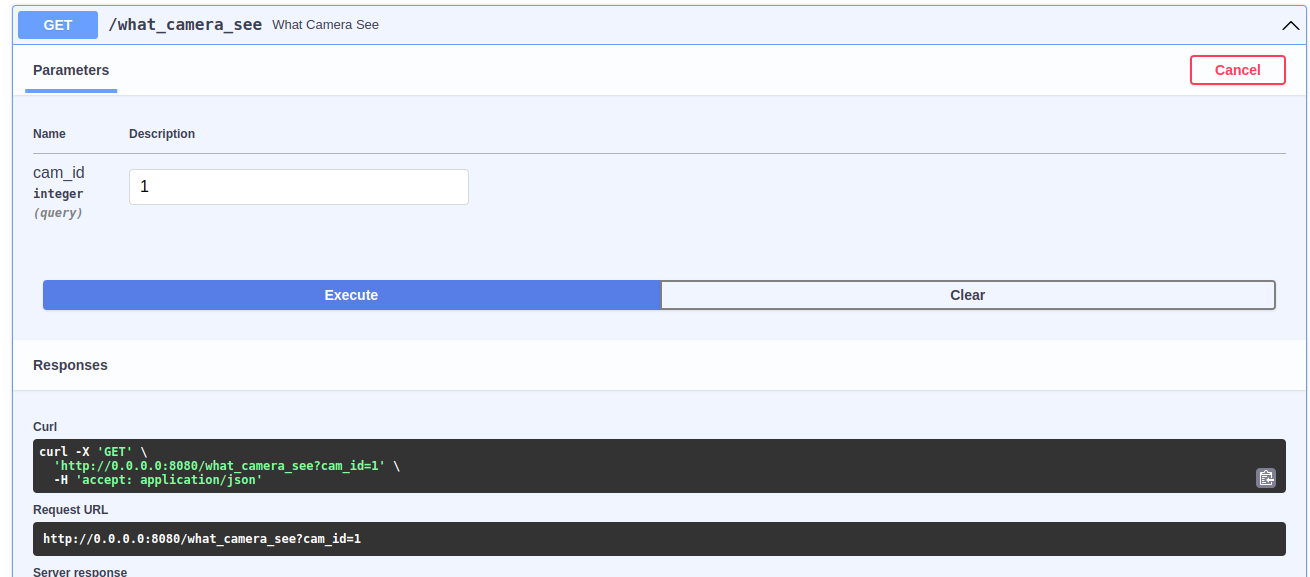
\includegraphics[width=0.9\linewidth]{assets/images/demon-1-cam.png}
	\caption{Демонстрация запроса}
	\label{fig:i:hate:niggers}
\end{figure}
\FloatBarrier

На рисунке \ref{fig:i:hate:niggers2} демонстрируется результат запроса, из которого видно, что камера видит трех посетителей, в виде json документа. 

\begin{figure}[ht!]
	\centering
	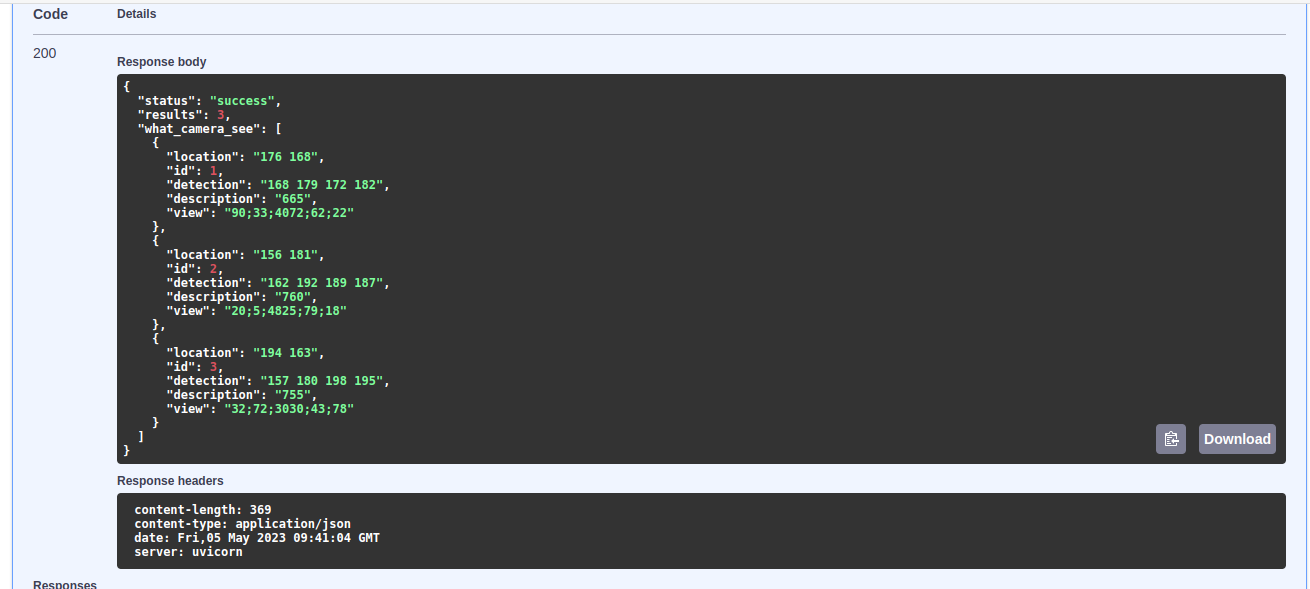
\includegraphics[width=0.9\linewidth]{assets/images/demon-2-cam.png}
	\caption{Демонстрация результата запроса}
	\label{fig:i:hate:niggers2}
\end{figure}
\FloatBarrier


\subsection{Постановка исследования}

Постановка исследования - это важный этап любого исследовательского проекта, который позволяет определить цели и задачи исследования, а также выбрать методы и инструменты для достижения поставленной цели.

В данном случае, целью исследования является изучение времени обработки операции от количества запросов в системе управления базами данных (СУБД). Эта цель может быть актуальна для предприятий и организаций, которые используют БД для хранения и обработки большого объема информации.

Исследование времени обработки операции от количества запросов в СУБД может быть полезным для оптимизации работы систем управления базами данных, а также для повышения эффективности работы с БД в целом. Полученные результаты могут помочь организациям выбрать наиболее подходящую СУБД и оптимальную структуру таблиц, а также определить оптимальное количество запросов для ускорения работы СУБД без потери качества данных.

Целью является исследование времени обработки операции от количества запросов в
СУБД.

\subsection{Результаты исследования}

В таблице \ref{tab:time1} продемонстрировано пользовательское время программы
при разном количестве полей таблиц.

\begin{table}[ht!]
	\begin{center}

		\caption{Время работы программы при разном
			количестве
			полей}
		\label{tab:time1}
		\begin{tabular}{|c|c|}
			\hline
			Количетво полей & Время в с. \\
			\hline
			100             & 0.006      \\
			\hline
			1000            & 0.009      \\
			\hline
			10000           & 0.097      \\
			\hline
			100000          & 1.170      \\
			\hline
			1000000         & 11.118     \\
			\hline

		\end{tabular}
	\end{center}
\end{table}
\newpage
На рисунке \ref{graph:r} представлено время запроса к БД.

\begin{figure}[ht!]
	\begin{center}
		\captionsetup{singlelinecheck = false,
			justification=centerfirst}
		\begin{tikzpicture}
			\begin{axis}[
					xlabel={Количетво полей},
					ylabel={время, с},
					width = 0.95\textwidth,
					height=0.3\textheight,
					xmin=0, xmax=100000,
					legend pos=north west,
					xmajorgrids=true,
					grid style=dashed,
				]
				\addplot[
					blue,
					semithick,
					mark = x,
					mark size = 3pt,
					thick,
				] file {assets/code/time.dat};

				\legend{
					Время работы программы
				}
			\end{axis}
		\end{tikzpicture}
		\centering
		\caption{Результаты время запроса к БД}
		\label{graph:r}
	\end{center}
\end{figure}

Из результатов исследования можно сделать вывод, что зависимость времени запроса от количества полей линейно.

\subsection*{Вывод}

В данном разделе постановлена задачи исследования и представлены результаты
данного исследования.